\documentclass[a4j,10pt,fleqn]{jsarticle}
\usepackage{atbegshi}
\AtBeginShipoutFirst{\special{pdf:tounicode 90ms-RKSJ-UCS2}}
\usepackage{txfonts,times}
%\usepackage{ascmac}
\usepackage{okumacro}
\usepackage{longtable}
\usepackage[dvipdfmx]{graphicx,xcolor}
\usepackage[dvipdfmx]{hyperref}
\usepackage{pxjahyper}

%%%
%この文書の組版は奥村晴彦さんの「pLaTeX2e 新ドキュメントクラス」を用いています。
%
%  http://www.matsusaka-u.ac.jp/~okumura/jsclasses/
%

\title{\textbf{文字コードとその実装}}
\author{荒川靖弘}
\date{第1版(公開版) 2001年11月3日}

%\AtBeginDvi{\special{pdf:tounicode 90ms-RKSJ-UCS2}}
\hypersetup{% Setup for hyperref packeage
    colorlinks=true,
    pdftitle=文字コードとその実装,
    pdfsubject=,
    pdfauthor=荒川 靖弘,
    pdfkeywords=JIS ISO2022 Unicode}

\begin{document}

\maketitle

\tableofcontents


\clearpage
\section{はじめに}

異なるプラットフォームでテキスト情報をやり取りする際に必ず問題になるのが
「文字コード」の変換です。
また近年はインターネットに代表される情報交換の「国際化」も意識されはじめ,
それを受けて登場したUnicodeとの互換性も問題になっています。
本テキストでは「文字コード」の問題について考えてみたいと思います。


\section{文字コード}

通常私達が「文字コード」と呼んでいるものは,実際には以下に示す2つの内容を含んでいます。
\begin{itemize}
\item 符号化文字集合(coded charactor set)
\item 文字エンコーディング(charactor encoding)
\end{itemize}
「符号化文字集合」とは,
その名の通り符号化(数値化)した文字の集合を示します。
「文字エンコーディング」とは符号化文字集合を情報処理用の「データ」に変換する方式を示します。
符号化されている文字情報を更にエンコーディング(符号化)するというのは一見奇妙に見えます。
どうしてそのようになっているのか見ていくことにしましょう。

\subsection{ISO/IEC 646 とIRV(US-ASCII)}

表\ref{tbl:US-ASCII}\,はインターネットの世界では俗に「US-ASCII」と呼ばれている文字コードです。

\begin{table}[htp]
\begin{center}\begin{tabular}{|c||c|c|c|c|c|c|c|c|}
    \hline
       & 0 & 1  & 2          & 3          & 4             & 5          & 6             & 7 \\ \hline \hline
    0  & ~ & ~  &            & \texttt{0} & \texttt{@}    & \texttt{P} & \texttt{`}    & \texttt{p} \\ \hline
    1  & ~ & ~  & \texttt{!} & \texttt{1} & \texttt{A}    & \texttt{Q} & \texttt{a}    & \texttt{q} \\ \hline
    2  & ~ & ~  & \texttt{"} & \texttt{2} & \texttt{B}    & \texttt{R} & \texttt{b}    & \texttt{r} \\ \hline
    3  & ~ & ~ & \texttt{\#} & \texttt{3} & \texttt{C}    & \texttt{S} & \texttt{c}    & \texttt{s} \\ \hline
    4  & ~ & ~ & \texttt{\$} & \texttt{4} & \texttt{D}    & \texttt{T} & \texttt{d}    & \texttt{t} \\ \hline
    5  & ~ & ~ & \texttt{\%} & \texttt{5} & \texttt{E}    & \texttt{U} & \texttt{e}    & \texttt{u} \\ \hline
    6  & ~ & ~ & \texttt{\&} & \texttt{6} & \texttt{F}    & \texttt{V} & \texttt{f}    & \texttt{v} \\ \hline
    7  & ~ & ~  & \texttt{'} & \texttt{7} & \texttt{G}    & \texttt{W} & \texttt{g}    & \texttt{w} \\ \hline
    8  & ~ & ~  & \texttt{(} & \texttt{8} & \texttt{H}    & \texttt{X} & \texttt{h}    & \texttt{x} \\ \hline
    9  & ~ & ~  & \texttt{)} & \texttt{9} & \texttt{I}    & \texttt{Y} & \texttt{i}    & \texttt{y} \\ \hline
    A  & ~ & ~  & \texttt{*} & \texttt{:} & \texttt{J}    & \texttt{Z} & \texttt{j}    & \texttt{z} \\ \hline
    B  & ~ & ~  & \texttt{+} & \texttt{;} & \texttt{K}    & \texttt{[} & \texttt{k}   & \texttt{\{} \\ \hline
    C  & ~ & ~  & \texttt{,}        & $<$ & \texttt{L}  & $\backslash$ & \texttt{l}         &   $|$ \\ \hline
    D  & ~ & ~  & \texttt{-} & \texttt{=} & \texttt{M}    & \texttt{]} & \texttt{m}   & \texttt{\}} \\ \hline
    E  & ~ & ~  & \texttt{.}        & $>$ & \texttt{N} & \texttt{\^{}} & \texttt{n} & \texttt{\~{}} \\ \hline
    F  & ~ & ~  & \texttt{/} & \texttt{?} & \texttt{O}   & \texttt{\_} & \texttt{o}             &   \\ \hline
\end{tabular}\end{center}
\caption{IRV/US-ASCII} \label{tbl:US-ASCII}
\end{table}

ASCII(American National Standard Code for Information Interchange)は
もともとANSI(American National Standards Institute)\footnote{
    \href{http://www.ansi.org/}{\texttt{http://www.ansi.org/}} 参照。
} 規格(ANSI X3.4)
として決められていました。

一方,ANSIとは独立にISO(International Organization for Standardization: 国際標準化機構)\footnote{
    \href{http://www.iso.org/}{\texttt{http://www.iso.org/}} 参照。
} でも各国用の文字コード規格「ISO/IEC 646」が作られました。
現在のASCII(US-ASCII)は ISO/IEC 646 のIRV(International Reference Version: 国際基準版)と同一となっています。
ISO/IEC 646 は7\,bitのコード空間を定義していて,
大まかに以下の4つの領域で構成されています。
(模式的に書くと表\ref{tbl:ISO646}\,のようになります)

\begin{enumerate}
\item 制御文字(control charactors): 00H~1FH
\item SP(SPACE): 20H
\item 図形文字(graphic characters): 21H~7EH
\item DEL(DELETE): 7FH
\end{enumerate}

\begin{table}[htp]
\begin{center}\begin{tabular}{|cc|cccccc|}
    \hline
       &   & \multicolumn{1}{c|}{\footnotesize{SP}} &   &   &   &   &   \\ \cline{3-3}
     ~ & ~ & ~ & ~ & ~ & ~ & ~ & ~ \\
       &   &   &   &   &   &   &   \\
       &   &   &   &   &   &   &   \\
       &   &   &   &   &   &   &   \\
    \multicolumn{2}{|c|}{\footnotesize{CL}} &   &   & \multicolumn{2}{c}{\footnotesize{GL}} &   &   \\
       &   &   &   &   &   &   &   \\
       &   &   &   &   &   &   &   \\
       &   &   &   &   &   &   &   \\
       &   &   &   &   &   &   &   \\
       &   &   &   &   &   &   &   \\  \cline{8-8}
       &   &   &   &   &   &   & \multicolumn{1}{|c|}{\footnotesize{DEL}} \\
    \hline
\end{tabular}\end{center}
\caption{ISO/IEC 646} \label{tbl:ISO646}
\end{table}

制御文字領域は「CL」とも呼ばれています。
SPは空白文字で図形文字の一種と考えることもできます。
図形文字(いわゆる「文字」)領域は「GL」とも呼ばれています。
DELはもともと紙テープ時代に削除用のコードとして使われていた時の名残のようです。
意味的には制御文字の一種と考えられなくもないですが,
制御文字としては定義されていません。
SPとDELはGLに含める場合があります。

ISO/IEC 646 は本来,符号化文字集合を定めたものですが,
実際にはそのコードをそのまま上記のようにエンコーディングして使っています。

\subsubsection{JISラテン文字} \label{sec:JISRoman}

日本では ISO/IEC 646 に相当するものとして JIS X 0201 ラテン文字が定義されています。
(JIS X 0201 については\ref{sec:JISX0201}章で改めて解説します)
IRVとJISラテン文字との違いは以下のとおりです。

\begin{quote}\begin{tabular}{|c||l|l|}
    \hline
    コード & IRV & JIS \\ \hline
    \hline
       5CH & $\backslash$(REVERSE SOLIDUS) & \texttt{\yen}(YEN SIGN) \\ \hline
       7EH & \texttt{\~{}}(TILDE)         & \texttt{\={}}(OVER LINE) \\ \hline
\end{tabular}\end{quote}

このように日本ではIRVとJISラテン文字の違いは僅かです。
しかし欧州などではIRVとの違いが顕著で各国間で全く互換が取れない状態になってしまいました。
その結果(日本を除く)殆どの国は ISO/IEC 646 の各国語バージョンを使わなくなり,
\ref{sec:ISO8859}章で述べる ISO/IEC 8859 や「コードページ」にシフトしていきました。


\subsection{ISO/IEC 8859 と JIS X 0201} \label{sec:ISO8859}

各国間の文字コードの不整合を緩和するため,
ISOでは ISO/IEC 646 のコード空間を8\,bitに拡張した規格
「ISO/IEC 8859」が作られました。
ISO/IEC 8859 のレイアウトは ISO/IEC 646 を2つ並べたような形になっています。
(模式的に書くと表\ref{tbl:ISO8859}\,のようになります)

\begin{enumerate}
\item CL制御文字(CL control charactors): 00H~1FH
\item GL図形文字(GL graphic characters): 20H~7FH(含むSP,DEL)または 21H~7EH
\item CR制御文字(CR control charactors): 80H~9FH
\item GR図形文字(GR graphic characters): A0H~FFH または A1H~FEH
\end{enumerate}

\begin{table}[htp]
\begin{center}\begin{tabular}{|cc|cccccc|cc|cccccc|}
    \hline
       &   & \multicolumn{1}{c|}{\footnotesize{~}} &   &   &   &   &   &   &   & \multicolumn{1}{c|}{\footnotesize{~}} &   &   &   &   &   \\ \cline{3-3} \cline{11-11}
     ~ & ~ & ~ & ~ & ~ & ~ & ~ & ~ & ~ & ~ & ~ & ~ & ~ & ~ & ~ & ~ \\
       &   &   &   &   &   &   &   &   &   &   &   &   &   &   &   \\
       &   &   &   &   &   &   &   &   &   &   &   &   &   &   &   \\
       &   &   &   &   &   &   &   &   &   &   &   &   &   &   &   \\
    \multicolumn{2}{|c|}{\footnotesize{CL}} &  \multicolumn{6}{c|}{\footnotesize{GL}} & \multicolumn{2}{c|}{\footnotesize{CR}} & \multicolumn{6}{c|}{\footnotesize{GR}} \\
       &   &   &   &   &   &   &   &   &   &   &   &   &   &   &   \\
       &   &   &   &   &   &   &   &   &   &   &   &   &   &   &   \\
       &   &   &   &   &   &   &   &   &   &   &   &   &   &   &   \\
       &   &   &   &   &   &   &   &   &   &   &   &   &   &   &   \\
       &   &   &   &   &   &   &   &   &   &   &   &   &   &   &   \\  \cline{8-8} \cline{16-16}
       &   &   &   &   &   &   & \multicolumn{1}{|c|}{\footnotesize{~}}  &   &   &   &   &   &   &   & \multicolumn{1}{|c|}{\footnotesize{~}} \\
    \hline
\end{tabular}\end{center}
\caption{ISO/IEC 8859} \label{tbl:ISO8859}
\end{table}

通常 ISO/IEC 8859 のCL,GL領域にはIRVがそのまま収容されます。
GR領域には各国特有の文字が割り当てられました。
ISO/IEC 8859 の実装で最も有名なのは ISO/IEC 8859-1(通称「Latin-1」)で,
フランス語やドイツ語などの西欧でよく使われる文字が収容されています\footnote{
    ISO/IEC 8859 は2001年3月現在,
    ISO/IEC 8859-1~10,13~15 が発行済になっています。
}。

各国間の文字コードの互換性に悩んでいた(特に)欧州では,ISO/IEC 8859 は広く受け入れられ,
現在もよく使われてます。

\subsubsection{JIS X 0201} \label{sec:JISX0201}

日本で ISO/IEC 8859 に相当するものとして JIS X 0201(当時は JIS C 6220 と呼ばれていました)があります。
JIS X 0201 ではラテン文字と片仮名を定義していて,
GLに(IRVではなく)ラテン文字,GRに片仮名を配置しています。
(表\ref{tbl:JISX0201-8}\,参照)

\begin{table}[htp]
\begin{center}\begin{tabular}{|c||c|c|c|c|c|c|c|c|c|c|c|c|c|c|c|c|}
    \hline
       & 0 & 1  & 2          & 3          & 4             & 5          & 6             & 7          & 8 & 9 & A  & B  & C  & D  & E & F \\ \hline \hline
    0  & ~ & ~  &            & \texttt{0} & \texttt{@}    & \texttt{P} & \texttt{`}    & \texttt{p} & ~ & ~ &    & ー & タ & ミ & ~ & ~ \\ \hline
    1  & ~ & ~  & \texttt{!} & \texttt{1} & \texttt{A}    & \texttt{Q} & \texttt{a}    & \texttt{q} & ~ & ~ & 。 & ア & チ & ム & ~ & ~ \\ \hline
    2  & ~ & ~  & \texttt{"} & \texttt{2} & \texttt{B}    & \texttt{R} & \texttt{b}    & \texttt{r} & ~ & ~ & 「 & イ & ツ & メ & ~ & ~ \\ \hline
    3  & ~ & ~ & \texttt{\#} & \texttt{3} & \texttt{C}    & \texttt{S} & \texttt{c}    & \texttt{s} & ~ & ~ & 」 & ウ & テ & モ & ~ & ~ \\ \hline
    4  & ~ & ~ & \texttt{\$} & \texttt{4} & \texttt{D}    & \texttt{T} & \texttt{d}    & \texttt{t} & ~ & ~ & 、 & エ & ト & ヤ & ~ & ~ \\ \hline
    5  & ~ & ~ & \texttt{\%} & \texttt{5} & \texttt{E}    & \texttt{U} & \texttt{e}    & \texttt{u} & ~ & ~ & ・ & オ & ナ & ユ & ~ & ~ \\ \hline
    6  & ~ & ~ & \texttt{\&} & \texttt{6} & \texttt{F}    & \texttt{V} & \texttt{f}    & \texttt{v} & ~ & ~ & ヲ & カ & ニ & ヨ & ~ & ~ \\ \hline
    7  & ~ & ~  & \texttt{'} & \texttt{7} & \texttt{G}    & \texttt{W} & \texttt{g}    & \texttt{w} & ~ & ~ & ァ & キ & ヌ & ラ & ~ & ~ \\ \hline
    8  & ~ & ~  & \texttt{(} & \texttt{8} & \texttt{H}    & \texttt{X} & \texttt{h}    & \texttt{x} & ~ & ~ & ィ & ク & ネ & リ & ~ & ~ \\ \hline
    9  & ~ & ~  & \texttt{)} & \texttt{9} & \texttt{I}    & \texttt{Y} & \texttt{i}    & \texttt{y} & ~ & ~ & ゥ & ケ & ノ & ル & ~ & ~ \\ \hline
    A  & ~ & ~  & \texttt{*} & \texttt{:} & \texttt{J}    & \texttt{Z} & \texttt{j}    & \texttt{z} & ~ & ~ & ェ & コ & ハ & レ & ~ & ~ \\ \hline
    B  & ~ & ~  & \texttt{+} & \texttt{;} & \texttt{K}    & \texttt{[} & \texttt{k}   & \texttt{\{} & ~ & ~ & ォ & サ & ヒ & ロ & ~ & ~ \\ \hline
    C  & ~ & ~  & \texttt{,}        & $<$ & \texttt{L} & \texttt{\yen} & \texttt{l}         &   $|$ & ~ & ~ & ャ & シ & フ & ワ & ~ & ~ \\ \hline
    D  & ~ & ~  & \texttt{-} & \texttt{=} & \texttt{M}    & \texttt{]} & \texttt{m}   & \texttt{\}} & ~ & ~ & ュ & ス & ヘ & ン & ~ & ~ \\ \hline
    E  & ~ & ~  & \texttt{.}        & $>$ & \texttt{N} & \texttt{\^{}} & \texttt{n} & \texttt{\={}} & ~ & ~ & ョ & セ & ホ & ゛ & ~ & ~ \\ \hline
    F  & ~ & ~  & \texttt{/} & \texttt{?} & \texttt{O}   & \texttt{\_} & \texttt{o}             &   & ~ & ~ & ッ & ソ & マ & ゜ & ~ & ~ \\ \hline
\end{tabular}\end{center}
\caption{JIS X 0201(8\,bit)} \label{tbl:JISX0201-8}
\end{table}

実は JIS X 0201 には7\,bitのエンコーディング方法も定義されています。
(これについては\ref{sec:JISX0201-7}章で解説します)
しかし,実際にはこの8\,bitエンコーディングの方が広く受け入れられました。

\subsubsection{コードページ}

一方,IBM/PC などでは「コードページ」という独自の体系が作られました。
これは(CL,CRの制御文字領域も含めた)8\,bit空間をフルに使って図形文字を割り当てたものです。
GL領域はほぼIRV(US-ASCII)ですがそれ以外は各国によって独自の図形文字が割り当てられています。
そして国別情報を表す情報として「コードページ」と呼ばれる値をPC内に保持しています。
日本語のページコードは「932」でほぼ JIS X 0201 に準拠した符号化がされています。
現在のDOS/Windowsシステムにもコードページは残っていて,
主に国別情報として使われています。


\subsection{ISO/IEC 2022 によるエンコーディング} \label{sec:ISO2022}

更にISOでは,符号化文字集合を動的に切り替え,複数バイト符号にも対応できるエンコーディング規格を作りました。
これが ISO/IEC 2022 です。
(ISO/IEC 2022 は日本では JIS X 0202 で定義されています)
図\ref{fig:ISO2022-8}\,は ISO/IEC 2022 のエンコーディングの仕組みを模式的に表したものです。

\begin{figure}[htp]
\begin{center}
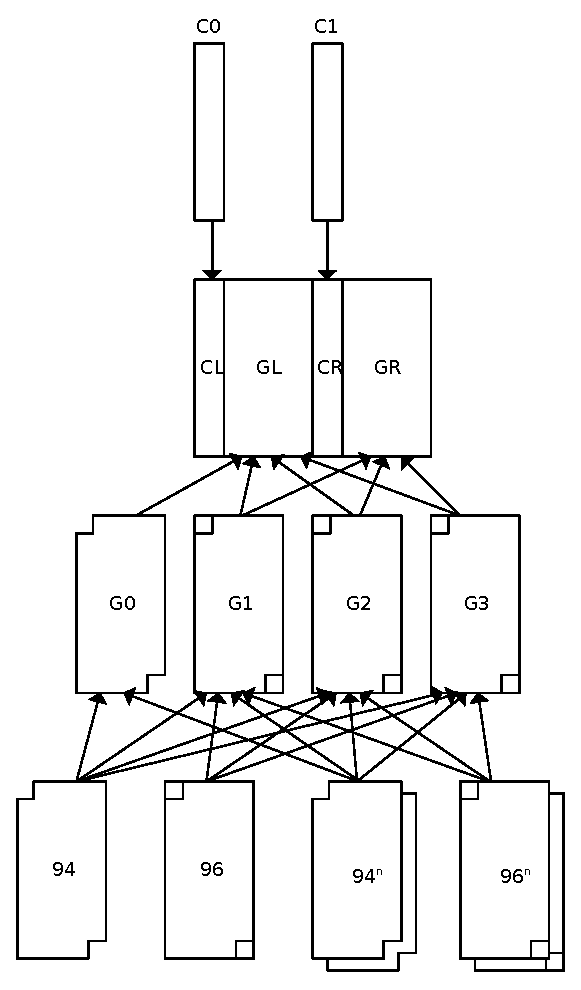
\includegraphics[width=7.5cm,clip]{iso2022-8.eps}
\end{center}
\caption{ISO/IEC 2022} \label{fig:ISO2022-8}
\end{figure}

これまでに登場した CL/CR/GL/GR で仕切られたコード空間を ISO/IEC 2022 では
「コードテーブル」(JIS X 0202 では「符号表」)と呼びます。
符号化された図形文字集合はコードテーブルに直接割り付けられるのではなく,
G0~G3の「中間バッファ」に一旦「指示」され,
中間バッファからコードテーブルのGLまたはGRに「呼び出」されます。
図形文字集合には従来の94または96文字集合の他,
複数バイト($94^{n}$または$96^{n}$)文字の集合にも対応しています。
ISO/IEC 2022 はCR/GRを使わないことで7\,bitエンコーディングにも対応できます。
中間バッファからコードテーブルへの「呼び出し」は「ロッキングシフト」と呼ばれ
C0/C1制御文字(\ref{sec:ctrl-charset}章参照)を使って行われます。
(ただし,LS0/LS1以外はエスケープシーケンスを用います)
表\ref{tbl:ISO2022-shift}\,にそのシーケンスを示します。
\begin{table}[htp]
\begin{center}\begin{tabular}{|l|l|l|}
    \hline
    ロッキングシフト & \multicolumn{2}{c|}{シーケンス} \\ \hline
    \hline
    SI/LS0(G0→GL) & 0FH      & \texttt{[SI]} \\ \hline
    SO/LS1(G1→GL) & 0EH      & \texttt{[SO]} \\ \hline
    LS2(G2→GL)    & 1BH 6EH  & \texttt{[ESC] n} \\ \hline
    LS3(G3→GL)    & 1BH 6FH  & \texttt{[ESC] o} \\ \hline
    LS1R(G1→GR)   & 1BH 7EH  & \texttt{[ESC] \~{}} \\ \hline
    LS2R(G2→GR)   & 1BH 7DH  & \texttt{[ESC] \}} \\ \hline
    LS3R(G3→GR)   & 1BH 7CH  & \texttt{[ESC] $|$} \\ \hline
\end{tabular}\end{center}
\begin{center}\begin{tabular}{|l|l|l|}
    \hline
    シングルシフト   & \multicolumn{2}{c|}{シーケンス} \\ \hline
    \hline
    SS2(G2→GL/GR) & 8EH または 1BH 4EH  & \texttt{[SS2]} または \texttt{[ESC] N} \\ \hline
    SS3(G3→GL/GR) & 8FH または 1BH 4FH  & \texttt{[SS3]} または \texttt{[ESC] O} \\ \hline
\end{tabular}\end{center}
\caption{ISO/IEC 2022 「呼び出し」シーケンス}\label{tbl:ISO2022-shift}
\end{table}%
なお,G0からGRへの呼び出しはできないことになっています。

シングルシフトは呼び出しの特別な形で,一時的に1文字だけ呼び出す場合に使用します。
シングルシフトはG2またはG3のみ使用でき,
通常はGLへ呼び出しますがGRへの呼び出しも可能です。

文字集合をG0~G3へ「指示」する場合もエスケープシーケンスを用います。
表\ref{tbl:ISO2022-req}\,に文字集合ごとの指示シーケンスを挙げます。
\begin{table}[htp]
\begin{center}\begin{tabular}{|r|l|l|}
    \hline
    指示             & \multicolumn{2}{c|}{シーケンス} \\ \hline
    \hline
    94文字集合 → G0 & 1BH 28H \textit{Ft} & \texttt{[ESC] ( \textit{Ft}} \\ \hline
    94文字集合 → G1 & 1BH 29H \textit{Ft} & \texttt{[ESC] ) \textit{Ft}} \\ \hline
    94文字集合 → G2 & 1BH 2AH \textit{Ft} & \texttt{[ESC] * \textit{Ft}} \\ \hline
    94文字集合 → G3 & 1BH 2BH \textit{Ft} & \texttt{[ESC] + \textit{Ft}} \\ \hline
    \hline
    96文字集合 → G1 & 1BH 2DH \textit{Ft} & \texttt{[ESC] - \textit{Ft}} \\ \hline
    96文字集合 → G2 & 1BH 2EH \textit{Ft} & \texttt{[ESC] .\ \textit{Ft}} \\ \hline
    96文字集合 → G3 & 1BH 2FH \textit{Ft} & \texttt{[ESC] / \textit{Ft}} \\ \hline
    \hline
    $94^n$文字集合 → G0 & 1BH 24H 28H \textit{Ft} または 1BH 24H \textit{Ft} & \texttt{[ESC] \$ ( \textit{Ft}} または \texttt{[ESC] \$ \textit{Ft}} \\ \hline
    $94^n$文字集合 → G1 & 1BH 24H 29H \textit{Ft} & \texttt{[ESC] \$ ) \textit{Ft}} \\ \hline
    $94^n$文字集合 → G2 & 1BH 24H 2AH \textit{Ft} & \texttt{[ESC] \$ * \textit{Ft}} \\ \hline
    $94^n$文字集合 → G3 & 1BH 24H 2BH \textit{Ft} & \texttt{[ESC] \$ + \textit{Ft}} \\ \hline
    \hline
    $96^n$文字集合 → G1 & 1BH 24H 2DH \textit{Ft} & \texttt{[ESC] \$ - \textit{Ft}} \\ \hline
    $96^n$文字集合 → G2 & 1BH 24H 2EH \textit{Ft} & \texttt{[ESC] \$ .\ \textit{Ft}} \\ \hline
    $96^n$文字集合 → G3 & 1BH 24H 2FH \textit{Ft} & \texttt{[ESC] \$ / \textit{Ft}} \\ \hline
\end{tabular}\end{center}
\caption{ISO/IEC 2022 「指示」シーケンス}\label{tbl:ISO2022-req}
\end{table}%
96文字集合または$96^n$文字集合をG0に指示することはできません。
$94^n$文字集合からG0への指示が2種類あるのは ISO/IEC 2022 の古い規格の名残です。
\textit{Ft} は符号化文字集合ごとに決められています。
主なものを表\ref{tbl:ISO2022-charset}\,に挙げます。
\begin{table}[htp]
\begin{center}\begin{tabular}{|l|c|l|}
    \hline
    種別          & \textit{Ft} & 符号化文字集合名 \\ \hline
    \hline
    94文字集合     & \texttt{@} & ISO/IEC 646 英国版 \\ \cline{2-3}
                   & \texttt{B} & ISO/IEC 646 IRV(US-ASCII) \\ \cline{2-3}
                   & \texttt{H} & スウェーデン名前文字 \\ \cline{2-3}
                   & \texttt{I} & JIS X 0201 片仮名 \\ \cline{2-3}
                   & \texttt{J} & JIS X 0201 ラテン文字 \\ \hline
    \hline
    96文字集合     & \texttt{A} & ISO/IEC 9959-1(GR部分) \\ \cline{2-3}
                   & \texttt{B} & ISO/IEC 9959-2(GR部分) \\ \cline{2-3}
                   & $\cdots$   & $\cdots$ \\ \hline
    \hline
    $94^n$文字集合 & \texttt{@} & JIS X 0208-1978(JIS C 6226) \\ \cline{2-3}
                   & \texttt{A} & GB 2312-80(中国語簡体字) \\ \cline{2-3}
                   & \texttt{B} & JIS X 0208-1983,1990,1997 \\ \cline{2-3}
                   & \texttt{C} & KS C 5601-1987(韓国語ハングル・漢字) \\ \cline{2-3}
                   & \texttt{D} & JIS X 0212-1990 \\ \cline{2-3}
                   & \texttt{O} & JIS X 0213 1面 \\ \cline{2-3}
                   & \texttt{P} & JIS X 0213 2面 \\ \hline
\end{tabular}\end{center}
\caption{ISO/IEC 2022 文字集合}\label{tbl:ISO2022-charset}
\end{table}

このように ISO/IEC 2022 は非常に柔軟性の高い(逆に言えば複雑な)規格なのですが,
この機能の全てを実装するのはあまり現実的ではありません。
そこで実際には ISO/IEC 2022 の一部を省略した「サブセット」が使われます。

日本では JIS X 0201,0208,0212,0213 各規格で ISO/IEC 2022 に対応する文字エンコーディングを定義しています。
JIS 0201 では,これまでも説明しましたが,ラテン文字と片仮名について定義しています。
JIS X 0208,0213 は漢字集合について定義したもので,
実装水準によって第一から第四まで決められています。
JIS X 0212 は「補助漢字」と呼ばれ,
もともと JIS X 0208 で不足している文字を補うために定義されたものですが,
あまり使われることはなく,
その後の JIS X 0213 の登場によって事実上obsolete(時代遅れ,破棄された)な規格となってしまいました。

\subsubsection{実装例: ISO/IEC 8859}

ISO/IEC 8859 は ISO/IEC 2022 に準拠したエンコーディングであると見なすことができます。
以下に簡単に概要を示します。
\begin{itemize}
\item G0にIRVを指示
\item G1に ISO/IEC 8859-x GR側を指示
\item G0をGLに呼び出す
\item G1をGRに呼び出す
\item 指示・呼び出し用のシーケンスは使わない
\end{itemize}

\subsubsection{実装例: JIS X 0201 7\,bitエンコーディング} \label{sec:JISX0201-7}

JIS X 0201 の8\,bitコーディングについては既に\ref{sec:JISX0201}章で説明しました。
JIS X 0201 の7\,bitコーディングについても ISO/IEC 2022 に準拠したコーディングがあります。
以下に概要を示します。
\begin{itemize}
\item G0に JIS X 0201 ラテン文字(またはIRV)を指示
\item G1に JIS X 0201 片仮名を指示
\item G0をGLに呼び出す
\item JIS X 0201 片仮名はG1をGLに呼び出すか直接G0に指示して使用
\item シングルシフトは使わない
\end{itemize}

この方法ならG0に他の符号化文字集合(JIS X 0208,0212,0213)を指示することでいくらでも拡張できます。
後述するISO-2022-JP(\ref{sec:iso-2022-jp}章)ではこのエンコーディング方法を拡張する形で実装されています。
(ただし厳密には ISO/IEC 2022 に準拠していません)

\subsubsection{実装例: ISO-2022-JP} \label{sec:iso-2022-jp}

ISO-2022-JPは\href{ftp://ftp.isi.edu/in-notes/rfc1468.txt}{RFC1468}\footnote{
    \href{http://www.asahi-net.or.jp/~bd9y-ktu/dtd_f/rfc_f/rfc1468j.html}{\texttt{http://www.asahi-net.or.jp/\~{}bd9y-ktu/dtd\_f/rfc\_f/rfc1468j.html}} 参照。
} で定められるメッセージ交換用の規格で,
JIS X 0208 の付属書でも言及されています。
ISO-2022-JP は ISO/IEC 2022 を参考に設計されていますが,
厳密に準拠していません。
これは主に\href{ftp://ftp.isi.edu/in-notes/rfc2822.txt}{RFC2822}\footnote{
    Internet Message Format: \href{http://www.puni.net/~mimori/rfc/rfc2822.txt}{\texttt{http://www.puni.net/\~{}mimori/rfc/rfc2822.txt}} 参照。
} (かつての\href{ftp://ftp.isi.edu/in-notes/rfc822.txt}{RFC822})に配慮したものです。
以下に概要を示します。
\begin{itemize}
\item 7\,bitエンコーディング固定
\item G0にIRV(US-ASCII)を指示
\item G0をGLに呼び出す
\item 文字集合の切り替えはG0への指示で行い,
    以下の符号化文字集合の組み合わせのみ許す(JIS X 0201 片仮名は許されていない)
    \begin{quote}\begin{tabular}{|l|l||l|}
        \hline
        1BH 28H 42H & \texttt{[ESC] ( B}  & ISO/IEC 646 IRV(US-ASCII) \\ \hline
        1BH 28H 4AH & \texttt{[ESC] ( J}  & JIS X 0201 ラテン文字 \\ \hline
        1BH 24H 40H & \texttt{[ESC] \$ @} & JIS C 6226-1978 \\ \hline
        1BH 24H 42H & \texttt{[ESC] \$ B} & JIS X 0208-1983,1990,1997 \\ \hline
    \end{tabular}\end{quote}
\item ロッキングシフト・シングルシフトは使わない
\item 改行コードを 0DH 0AH(\texttt{[CR] [LF]})とする。
\item テキストはIRVで始まる
\item 行末(改行コードの手前)は必ずIRVまたは JIS X 0201 ラテン文字になっていること
\item テキストは必ずIRVで終わらなければならない
\end{itemize}

更に\href{ftp://ftp.isi.edu/in-notes/rfc1554.txt}{RFC1554}\footnote{
    \href{http://www.asahi-net.or.jp/~bd9y-ktu/dtd_f/rfc_f/rfc1554j.html}{\texttt{http://www.asahi-net.or.jp/\~{}bd9y-ktu/dtd\_f/rfc\_f/rfc1554j.html}} 参照。
} ではISO-2022-JPを拡張した「ISO-2022-JP-2」を定義していて,
JIS補助漢字(JIS X 0212)や中国語簡体字,韓国語を指示することができます。
また ISO/IEC 8859 の文字セットをG2に指示し,シングルシフトで呼び出すことができるようにもなっています。
おそらくこれはUnicode(\ref{sec:Unicode}章参照)を意識したエンコーディングと考えられなくもないですが,
実際には殆ど見かけません。

ところで,
JIS X 0213 では「ISO-2022-JP-3\footnote{
    \href{http://www.asahi-net.or.jp/~wq6k-yn/code/enc-x0213.html}{\texttt{http://www.asahi-net.or.jp/\~{}wq6k-yn/code/enc-x0213.html}} 参照。
}」が定義されています。
ISO-2022-JP-3では以下の符号化文字集合を指示できます。
\begin{quote}\begin{tabular}{|l|l||l|}
    \hline
    1BH 28H 42H     & \texttt{[ESC] ( B}    & ISO/IEC 646 IRV(US-ASCII) \\ \hline
    1BH 24H 42H     & \texttt{[ESC] \$ B}   & JIS X 0213 1面(ISO-2022-JP互換用) \\ \hline
    1BH 24H 28H 4FH & \texttt{[ESC] \$ ( O} & JIS X 0213 1面 \\ \hline
    1BH 24H 28H 50H & \texttt{[ESC] \$ ( P} & JIS X 0213 2面 \\ \hline
\end{tabular}\end{quote}
JIS X 0213 の1面\footnote{
    JIS X 0213 は JIS X 0208 と共に使うことが前提となっています。
    JIS X 0208 の符号化文字集合は94区$\times$\,94点の2次元構成でしたが,
    JIS X 0213 では2面$\times$\,94区$\times$\,94点の3次元構成になっています。
} は従来のJIS漢字第一・第二水準(JIS X 0208)と今回新しく追加されたJIS漢字第三水準までを含んだ集合で,
2面はJIS漢字第四水準で追加された文字集合です。
更に現在広く使われているISO-2022-JPとの互換性を保つために
「\texttt{[ESC] \$ B}」の指示シーケンスを1面として認めています。
ただしこの場合には一部の文字が使えません。

ISO-2022-JP-3はまだRFC化されていないようですが,
一部のプラットフォームでは既に使われはじめています。

\subsubsection{実装例: EUC-JP} \label{sec:euc-jp}

EUC(Extended UNIX Code)は,文字通りUNIX系プラットフォームにおいて多言語化の一環として開発されました。
EUCの日本語サブセットのことを日本語EUCまたはEUC-JPと呼びます。
EUCも ISO/IEC 2022 に基づいて設計されています。
EUC-JPを例にとってみます。
\begin{itemize}
\item G0にIRV(または JIS X 0201 ラテン文字)を指示
\item G1に JIS X 0208 を指示
\item G2に JIS X 0201 片仮名を指示
\item G3に JIS X 0212 を指示
\item G0をGLに,G1をGRに呼び出す
\item G2とG3はシングルシフトで使用
\item ロッキングシフトは使わない
\end{itemize}

指示が固定で呼び出しのためのロッキングシフトを使わないので,
非常にすっきりしたコード体系になっているのが特徴です。
ただし,EUC-JPでは JIS X 0201 片仮名が冷遇されていて,
シングルシフトを含めた2\,byteコードになっています。
実際,
つい最近まで JIS X 0201 片仮名や JIS X 0212 の補助漢字を実装していない
UNIX系プラットフォームが多く存在していたそうで,
それがISO-2022-JPにおいて JIS X 0201 片仮名が排除された原因のひとつだとも言われています。

EUC-JPにも JIS X 0213 において対応するエンコーディング(EUC-JISX0213)が定義されています。
この場合は
G1に JIS X 0213 の1面を,
G3に JIS X 0213 の2面を指示します。

\subsubsection{制御文字集合} \label{sec:ctrl-charset}

ところで,今まで殆ど触れませんでしたが,
制御文字集合は ISO/IEC 6429(日本では JIS X 0211)で定義されています。
よく使われているものを表\ref{tbl:control-codes}\,に挙げます。
\begin{table}[htp]
\begin{center}\begin{tabular}{|c|c|c|l|}
    \hline
    形式 & \multicolumn{3}{c|}{制御文字} \\ \hline
    \hline
    C0   & 00H & NUL    & NULL(空) \\ \cline{2-4}
         & 08H & BS     & BACKSPACE(後退) \\ \cline{2-4}
         & 09H & HT     & CHARACTER TABULATION(文字タブ) \\ \cline{2-4}
         & 0AH & LF     & LINE FEED(改行) \\ \cline{2-4}
         & 0CH & FF     & FORM FEED(書式送り) \\ \cline{2-4}
         & 0DH & CR     & CARRIAGE RETURN(復帰) \\ \cline{2-4}
         & 0EH & SO/LS1 & SHIFT-OUT(シフトアウト)/LOCKING-SHIFT ONE(ロッキングシフト1) \\ \cline{2-4}
         & 0FH & SI/LS0 & SHIFT-IN(シフトイン)/LOCKING-SHIFT ZERO(ロッキングシフト0) \\ \cline{2-4}
         & 1BH & ESC    & ESCAPE(エスケープ) \\
    \hline
    C1   & 8EH & SS2    & SINGLE-SHIFT TWO(シングルシフト2) \\ \cline{2-4}
         & 8FH & SS3    & SINGLE-SHIFT THREE(シングルシフト3) \\
    \hline
\end{tabular}\end{center}
\caption{主な制御文字}\label{tbl:control-codes}
\end{table}%

このうちESCは特別な制御文字で,C0が呼び出されない状態でも有効になっています。
BSは合成文字(「\^a」など)を表現する際に使われるのですが,
プラットフォームによって対応していないことが多く,あまり使われません。
(ISO-2022-JPなどでは使ってはいけないことになっています)

\href{ftp://ftp.isi.edu/in-notes/rfc2822.txt}{RFC2822}でも定義されている制御文字があります。
NULは許されないコードとして定義されています。
CR/LFが連続して現れる場合は改行コードと見なされます。
更にHTおよびFFはMIME\footnote{
    \href{ftp://ftp.isi.edu/in-notes/rfc2046.txt}{RFC2046}(\href{http://www.asahi-net.or.jp/~bd9y-ktu/dtd_f/rfc_f/rfc2046j.html}{\texttt{http://www.asahi-net.or.jp/\~{}bd9y-ktu/dtd\_f/rfc\_f/rfc2046j.html}} 参照)。
} において「事実上の標準」となっています。


\subsection{シフトJIS} \label{sec:shiftJIS}

シフトJISはDOS/WindowsやMacintoshなどで使われるコード体系で,
商業的に大きなシェアを占めています。
シフトJISの起源は日本初の16\,bitパソコンである三菱の「Multi16」に搭載された
CP/M-86の日本語対応版に実装されたものであると言われています。
処理の容易なコードとしてMicrosoftなど数社が策定したもので,
「MS漢字コード」とも呼ばれています。

シフトJISは ISO/IEC 2022 非準拠です。
簡単にいうと JIS X 0201 8\,bit空間(表\ref{tbl:JISX0201-8}\,参照)の空いてる領域
(CRの全てとGRの使われていない領域)
に JIS X 0208 を無理矢理詰め込んだような構成になっています。
しかも,漢字コードの2\,byte目はGLの一部を含んでいます。

シフトJISは(当時としては)非常に巧妙にできていて,
(漢字の使えなかった)旧来のシステムとの整合性もよく,
日本国内で急速に広まっていきました。
しかし文字集合を無理矢理に詰め込んでいるため,拡張性に乏しいのが難点です。
実際に補助漢字である JIS X 0212 はシフトJISに取り込まれませんでした。
なお新しくできた JIS X 0213 では,JIS X 0212 の反省を踏まえ,
シフトJIS用のエンコーディング(Shift\_JISX0213)も提供しています。

シフトJISが今後の国際化・多言語化に対応しきれないのは明らかであり,
新しいコード体系へのシフトが求められています。


\subsection{ISO/IEC 10646-1(Unicode)} \label{sec:Unicode}

1984年,ISOは文字コードの国際化(I18N: InternationalizatioN)を図るため,
全世界の主要な文字を含んだ単一の符号化文字集合 ISO/IEC 10646 の策定を開始しました。
この作業が始まった同じ頃米国の有力なコンピュータ企業が集まって
同じような符号化文字集合「Unicode\footnote{
    \href{http://www.unicode.org/}{\texttt{http://www.unicode.org/}} 参照。
}」を開発しました。
最終的には,両者の歩み寄りにより,
「ISO/IEC 10646-1」に統合されました。
日本では JIS X 0221 で定義されています。

ISO/IEC 10646-1 の符号化文字集合のことを特に
「UCS」(Universal Multiple-Octet Coded character Set)と呼びます。
またエンコーディングのことを
「UTF」(UCS Transfer Format)と呼びます。

\subsubsection{UCS}

UCSには現在「UCS-2」と「UCS-4」があります。

UCS-4は ISO/IEC 10646-1 が定義するフルサイズ(31\,bit)のコード空間で
群(group)・面(plane)・区(row)・点(cell)の4次元構成になっています。
256区$\times$\,256点で1つの面を構成し,
更に256面で1つの群を構成しています。
群は128あります。

00群00面を特に「BMP」(Basic Multilingual Plane: 基本多言語面)と呼んでいます。
現時点で定義されている文字集合は全てBMPに収められており,
他の群・面には何も定義されていません。
このBMPを16\,bitで符号化したものがUCS-2です。
(もともとのUnicodeはUCS-2のみ定義していました。
従ってUnicodeは ISO/IEC 10646-1 のサブセットであるということもできます)

\subsubsection{UTF}

現在よく使われるUTFとしては
「UTF-16」,「UTF-8」,「UTF-7」があります。

UTF-16は基本的にはUCS-2の符号をそのままコードとして使っています。
ただし拡張用に,BMPに続く16面分を埋めこむことのできる
「Surrogate Pair」という仕組みを持っています。

UTF-8はUCSを ISO/IEC 2022 と整合性のある方法でエンコードしたものです。
すなわち,UCSのIRVに相当する文字集合をGLに,
残りの文字を2~6\,byteの可変サイズの$96^n$文字集合としてGRに配置します。
従来のエンコーディングとの(特にGLにおいて)衝突が少ないため,
UTF-8は広く受け入れられています。
特にオープンソース・コミュニティでは事実上の国際標準コードとなりつつあります。

UTF-7はUTF-8を(電子メールのような)7\,bit伝送系でも通せるように(Base64のような方法で)変換したものです。
一般にはあまり使われませんが,
8\,bitデータを扱えない特殊な条件下では使われることがあります。


\section{文字コードにまつわる諸問題}

日本では符号化文字集合はJISで統一されているかのように見えますが,
互換性などにおいて様々な問題を抱えています。
これに加え,多様な文字エンコーディングが更に問題を複雑にしています。
この章ではそういった問題点を具体的な事例を示しながら紹介していきます。


\subsection{IRVとJISラテン文字}

前述(\ref{sec:JISRoman}章)したとおり,
IRVとJISラテン文字の違いはわずか2字です。
これは日本国内に限ってはあまり問題がないように思えますが,
「国際化」を考える際には大きな問題になります。

まず「\texttt{\~{}}」(TILDE)と「\texttt{\={}}」(OVER LINE)ですが,
JIS X 0201 の附属書2では(送受信者間で合意があれば)両者を区別しないとしています。
Windows等では日本語環境でも7EHが「\texttt{\~{}}」になっています。
しかし一方で,ISO/IEC 10646-1 では両者は厳密に区別されています。

現実には「\texttt{\~{}}」や「\texttt{\={}}」を単独で意味ある文字として使うことはまずありません。
「\texttt{\~{}}」や「\texttt{\={}}」は制御記号として使われることが多く,
それ以外では合成文字の要素(「\~a」の「\~{}」など)として使われる程度です。
しかも昨今では合成文字は(互換性の問題から)殆ど使われませんし,
そういう意味では字形にこだわる必要はないのかもしれません。
しかし,ISO/IEC 10646-1 で明確に区別されている以上どちらかを選ぶ必要があり,
その「選択」を巡って混乱が起きることは必至です。

「$\backslash$」(REVERSE SOLIDUS)と「\texttt{\yen}」(YEN SIGN)では更に深刻です。
例えばC言語のプログラミングで日本円で金額を表示したい時,UCSを使ってコーディングするなら次のようになる筈です。
\begin{quote}\begin{tabular}{rl}
    コーディング: & \texttt{printf("Total: {\yen}\%d.{$\backslash$}n", maney);} \\
          出力例: & \texttt{Total: {\yen}646.} \\
\end{tabular}\end{quote}%
しかし,(UCSを使わない)これまでのコードはこのように区別されていません。
JISラテン文字を実装する日本語圏のシステムなら次のようにコーディングされているでしょう。
\begin{quote}\begin{tabular}{rl}
    コーディング: & \texttt{printf("Total: {\yen}{\yen}\%d.{\yen}n", maney);} \\
          出力例: & \texttt{Total: {\yen}646.} \\
\end{tabular}\end{quote}%
このコードをJISラテン文字を実装していない,例えばIRVのみのシステムに適用すると,
出力結果は本来意図したものとは違うものになる筈です。
\begin{quote}\begin{tabular}{rl}
    コーディング: & \texttt{printf("Total: {$\backslash$}{$\backslash$}\%d.{$\backslash$}n", maney);} \\
          出力例: & \texttt{Total: {$\backslash$}646.} \\
\end{tabular}\end{quote}%

国際化の流れの中ではJISラテン文字は使われなくなる傾向にあります。
(例えばISO-2022-JP-3ではJISラテン文字は定義されていません)
従って今後JISラテン文字固有の文字(「\texttt{\yen}」「\texttt{\={}}」)を意味ある文字として使う際は,
何らかの代替え手段
(JIS漢字集合を用いるか文字集合全体をUCS/UTFでエンコードする)
を講じる必要があります。


\subsection{「半角カナ」について} \label{sec:zen-han}

JIS X 0201 片仮名のことを俗に「半角カナ」といいます。
初期のキャラクタベース端末で表示されるデザインからそう呼ばれているようです。
日本のコンピュータ初期の時代では広く使われていましたが,
これも最近の国際化の流れの中で使われなくなりつつあります。

まずインターネットの黎明期における混乱が発端といえるでしょう。
当時インターネットの国内の前身であるJUNETはUNIX系プラットフォームをメインに使っていましたが,
当時のシステムは「半角カナ」を実装するものが少なかったといわれています。
(\ref{sec:euc-jp}章参照)
更にISOに「半角カナ」の指示コードを申請する際に,
当時は「H」で申請していたそうですが結局このコードは別のセットになり
(表\ref{tbl:ISO2022-charset}\,参照),
「半角カナ」は別のコード「I」に決まりました。
しかし日本国内ではこのことによる混乱が収まらず,
結局ISO-2022-JPでは「半角カナ」を使ってはいけないことに決まってしまいました。

JIS X 0208 附属書1ではシフトJISの「半角カナ」を将来削除する予定であると謳っていて,
JIS X 0213 でも「JIS X 0201 片仮名は原則として使わない」ことになっています。
(ISO-2022-JP-3では「半角カナ」は定義されていません)

JIS X 0201 のラテン文字および片仮名を総称して「半角文字」と呼ぶことがあります。
これに対し JIS X 0208,0212,0213 の漢字集合を「全角文字」と呼びます。
「全角文字」集合は「半角文字」の字形を含んでいて,これが特に国内において混乱の元になることがあります。
更に ISO/IEC 10646-1 ではこの「通称」に配慮して
「Halfwidth and Fullwidth Forms」という互換用の領域を作ってしまいました。
これには「半角カナ」と「全角英数字」が収められていて,
しかもJISラテン文字にない ISO/IEC 646 の各国語の文字の一部まで「全角英数字」として収容されています。

半角/全角の問題は,特に ISO/IEC 10646-1 も含めて考えると将来深刻な混乱を引き起こしかねません。
メッセージシステムを設計・運用する際には相当な注意が必要です。
なお「半角」と「全角」で字形が重複するものについては,
JISの各規格において以下の指針が与えられています。
\begin{itemize}
\item 「半角カナ」は使わず,「全角文字」で代替えする
\item 「半角カナ」は漢字集合を含んだエンコーディングとしては将来廃止される。
\item 「英数字」においてIRVで定義される文字と同一のものについては「全角文字」を使用しない
\end{itemize}


\subsection{旧JIS漢字と新JIS漢字}

JIS X 0208 は1983年に大改定されました。
1983年以前のJIS漢字集合(JIS C 6226-1978\footnote{
    JIS X 0208 はそれまで JIS C 6226 と呼ばれていました。
})を「旧JIS」,
1983年以降のJIS漢字集合(JIS X 0208,0212,0213)を「新JIS」と呼びます。
この大改定は主に字体や字形の変更や交換を行うものでしたが,
コンピュータ界に大きな混乱をもたらしました。
現在は殆どのプラットフォームで新JISへの移行が完了していますが,
これにより逆に旧JISで書かれたテキストが「文字化け」することになってしまいました。

最も顕著な例はISO-2022-JPです。
ISO-2022-JPでは旧JISを許容していて旧JISと新JISの混在するテキストを書くことも可能です。
しかし旧JISのセットを持っていない処理系では,旧JIS部分も無理矢理新JISで表示せざるをえません。
またISO-2022-JP以外のエンコーディングでは旧JISと新JISを区別できないため,
ISO-2022-JPから他のエンコーディングに変換する際に旧JISの情報が失われてしまいます。

このような混乱を回避するため,特に電子メールにおいては,
以下のようなローカルルールがあります。
\begin{itemize}
\item JIS漢字集合を使う際は新JISを指示(1BH 24H 42H)する
\item 1\,byte文字を使う際はIRVを指示(1BH 28H 42H)する
\item JISラテン文字および旧JISは使用しない
\end{itemize}%
これは\href{ftp://ftp.isi.edu/in-notes/rfc1468.txt}{RFC1468}には記載されていませんが,
JIS漢字を含むメールをやり取りを行う際の暗黙のルールになっています。


\subsection{ベンダ固有文字}

最初の JIS X 0208(JIS C 6226-1978)以前はメーカごとに文字コードを策定していました。
JIS漢字制定後もそれまでの文字コードとの互換性を確保するため,JIS漢字の不足分を独自に追加しています。
これが「ベンダ固有文字」です。
「機種依存文字」とか「システム外字」とか呼ばれることもあります。
ベンダ固有文字としては以下の2つが有名です。
\begin{quote}\begin{description}
\item[IBM拡張文字] :\par
    IBMが自社のメインフレームの文字集合から JIS C 6226-1978 でカバーされない文字を選んだもの。
\item[NEC拡張文字] :\par
    NECがIBM拡張文字に加えてさらに記号類や半角文字を追加したもの。
    俗に言う「98文字」。
\end{description}\end{quote}
これらの文字は JIS C 6226-1978 の符号化文字集合の空き領域(1面の9~15区・85~94区および2面\footnote{
    シフトJISでは2\,byte文字の第1\,byteが
    85H~88H・EBH~FFHの範囲にある領域にあたります。
})に配置されていて,
JIS C 6226-1978 で収容されなかった記号や漢字の異体字などが収められています。

ベンダ固有文字の定義はベンダやプラットフォームごとに違っていて,殆ど互換性がありません。
JIS規格でも情報交換用としてはベンダ固有文字などのJIS未定義文字を使うことを禁じています。
しかし,ユーザの立場では使っている文字がベンダ固有文字かどうか(特に異体字は)見た目でわかりにくく,
しばしば混乱の元になっています。

JIS X 0213 ではこれらのベンダ固有文字を含めた形で符号化文字集合が定義されています。
異体字についても包摂\footnote{
    JIS漢字には「包摂規準」というのがあり,
    意味が同じで似た字形の漢字を「同じ字体」とみなすことになっています。
    異体字の殆どはあるひとつの字体に包摂されるため,JIS漢字として収容されません。
} の例外としてかなりの数が新たに追加されているようです。
今後 JIS X 0213 がどの程度普及するか分かりませんが
(現在UNIX系プラットフォームを中心に整備されつつあります),
JIS X 0213 と情報交換用のエンコーディングであるISO-2022-JP-3が定着すれば,
ベンダ固有文字に対する考え方が変わるかもしれません。

一方 ISO/IEC 10646-1 ではベンダ固有文字および JIS X 0213 漢字集合の殆どが既に収容されています\footnote{
    JIS X 0213 漢字集合のうち ISO/IEC 10646-1 に収容されていない文字は360字程あるそうです。
}。
したがって,電子メールなどでもエンコードをUTF-8/UTF-7とすれば,
ベンダ固有文字と言われていた文字も使うことができます。


\section{おわりに}

本テキストでは「文字コード」の問題について一通り紹介しました。
実際には「文字」や「文字コード」の問題はこれだけではなく,
漢字の包摂と異体字の問題やUnicodeにおける「CJK統合」問題など色々ありますが,
「情報交換」において問題になりそうなところを中心に挙げていきました。
今回は問題を提示するだけでしたが,
電子メールなど異なるプラットフォーム間でのメッセージシステムを設計・運用する際の参考になると思います。

なお,文字コードについての文献を末尾に挙げていますが,
インターネット上でもいくつか情報があります。
主なものを以下に挙げます。
是非参考にしてください。
\begin{itemize}
\item 「文字コードの世界」(\href{http://euc.jp/i18n/charcode.ja.html}{\texttt{http://euc.jp/i18n/charcode.ja.html}})
\item 「従来の文字コードとUnicodeの対応に関する諸問題」(\href{http://euc.jp/i18n/ucsnote.ja.html}{\texttt{http://euc.jp/i18n/ucsnote.ja.html}})
\item 「JISとISO-2022」(\href{http://www.d2.dion.ne.jp/~imady/kcode/kcode_jis.html}{\texttt{http://www.d2.dion.ne.jp/\~{}imady/kcode/kcode\_jis.html}})
\item 「Mewニュースレター: ASCII」(\href{http://www.mew.org/Newsletters/6.html}{\texttt{http://www.mew.org/Newsletters/6.html}})
\item 「JIS X 0213 の代表的な符号化方式」\par
    (\href{http://www.asahi-net.or.jp/~wq6k-yn/code/enc-x0213.html}{\texttt{http://www.asahi-net.or.jp/\~{}wq6k-yn/code/enc-x0213.html}})
\end{itemize}


\nocite{Book:JISHandbook}\nocite{Book:CharCode}\nocite{Book:CharCode2}


\bibliographystyle{jplain}
\bibliography{charset}

\end{document}
